\documentclass{article}
\usepackage{multirow}
\usepackage{graphicx}
\title{Exercise 5\\System On Chip}
\author{Ole Magnus Ruud\\Vegar K\aa sli}
\begin{document}
\maketitle{}
\section{Scenarios}
\begin{center}
  \begin{tabular}{|r|p{8cm}|}
    \hline
\multicolumn{2}{|c|}{Use case scenario 1}\\\hline
Name:&Successful search for the right button order\\\hline
Context:&Top-level mode\\\hline
Pre-conditions:&Memory Machine is in initial state, no lights lit\\\hline
Post-conditions:&All lights are lit\\\hline
Start/Trigger:&User pushes a button\\\hline
Actors:&User, Memory Machine\\\hline
Description:&The user tries out pushing several buttons until one is lit. She then
    tries pushing another button causing the light to go out. She remembers
    the button that lit the first light and pushes this again, trying another
    second button. This time it is the right one, and the user continues in this
    fashion until she finds the complete correct button sequence and all the lights
    are lit\\\hline

  \end{tabular}
\end{center}


\begin{center}
  \begin{tabular}{|r|p{8cm}|}
    \hline
\multicolumn{2}{|c|}{Use case scenario 2}\\\hline
Name:&Unsuccessful search for the right button order\\\hline
Context:&Top-level mode\\\hline
Pre-conditions:&Memory Machine is in initial state, no lights\\\hline
Post-conditions:&No lights are lit\\\hline
Start/Trigger:&User pushes a button\\\hline
Actors/Roles:&User, Memory Machine\\\hline
Description:&
    The user tries out pushing several buttons until one is lit. He then
    tries pushing another button causing the light to go out. He remembers 
    the button that lit the first light and pushes this again, trying another
    second button. This time it is the right one, and he tries one more button
    which causes the lights to go out. This time he fails to remember the 
    first two buttons, and his frustration makes him give up.\\\hline

  \end{tabular}
\end{center}

\section{Sequence diagrams}
The following sequence diagrams outlines the communication between objects.
In this example, instances of Button classes and an instance of the Controller
class communicate with each other through the functions push() and light(). The
first sequence diagram(figure \ref{fig:seq1}) outlines scenario 1, 
while the second(figure \ref{fig:seq2}) outlines scenario
2. Both described as use cases in part 1.

  \begin{figure}
    \centering
  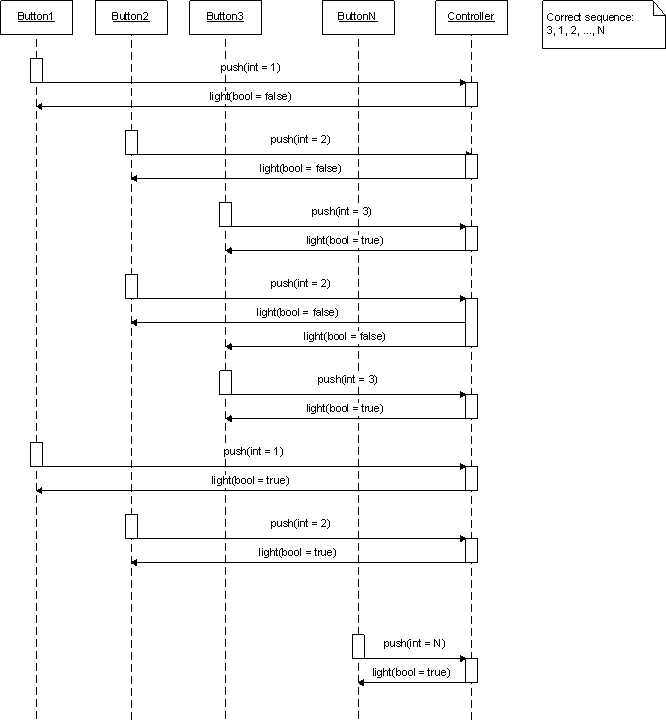
\includegraphics[width=\linewidth]{../sequence_scenario1}
    \caption{Sequence diagram, scenario 1}
    \label{fig:seq1}
  \end{figure}
  \begin{figure}[htbp]
    \centering
  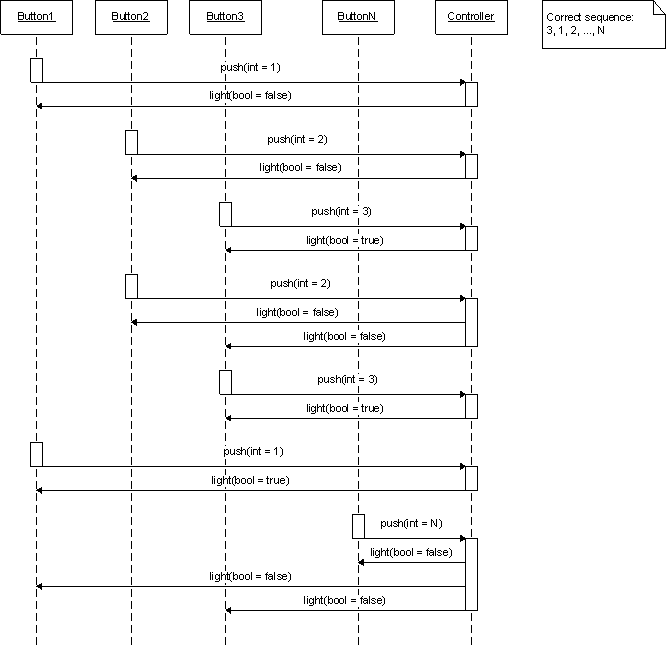
\includegraphics[width=\linewidth]{../sequence_scenario2}
    \caption{Sequence diagram, scenario 2}
    \label{fig:seq2}
  \end{figure}

\section{Class, objects and collaborations}
The class diagrams(figure \ref{fig:class1} and \ref{fig:classex4}) illustrates the 
structure of the systems from exercise 2 and 4, respectively.
The inclusion of Collaboration uses(figure \ref{fig:collabex2} 
and \ref{fig:collabex4}) and the composite 
structure diagram(figure \ref{fig:compex2} and \ref{fig:compex4}) 
defines the roles of the parts and their connections.
\begin{figure}[htbp]
  \centering
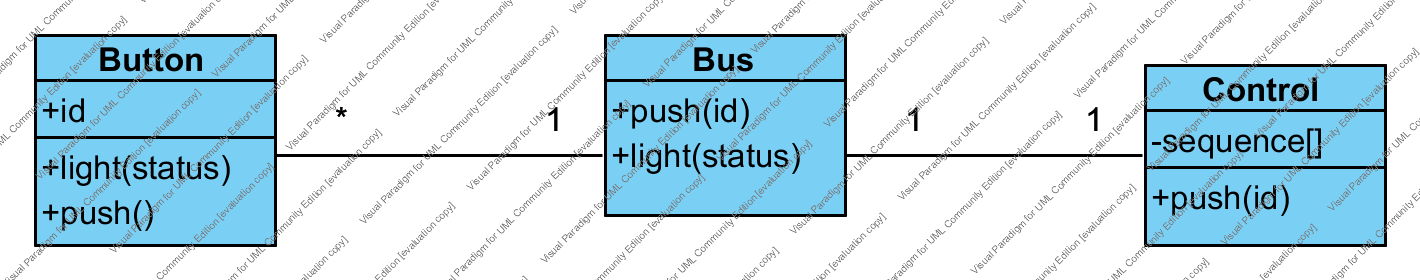
\includegraphics[width=\linewidth]{../class1}
  \caption{Class diagram, system from exercise 2}
  \label{fig:class1}
\end{figure}

\begin{figure}[htbp]
  \centering
  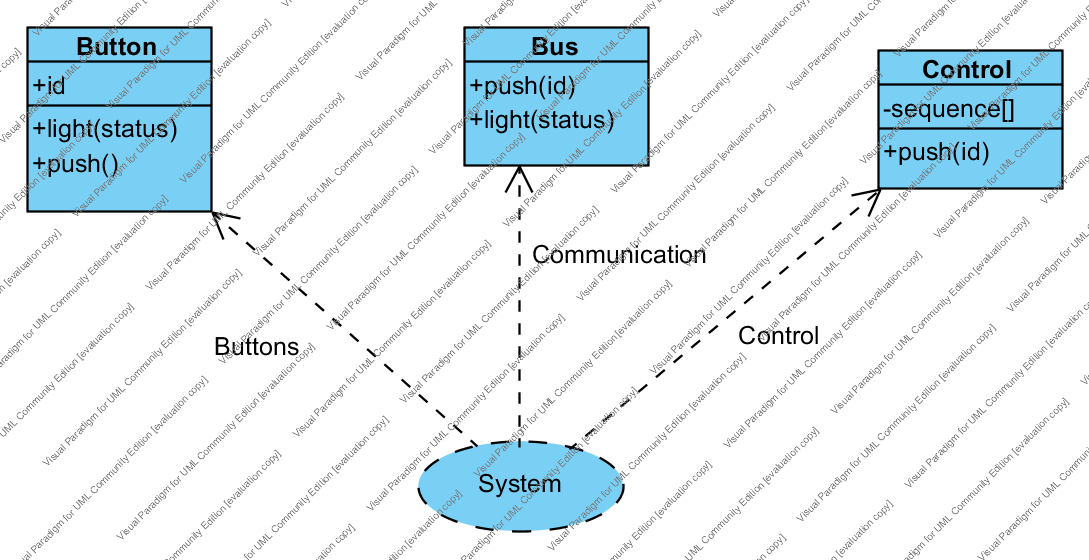
\includegraphics[width=\linewidth]{../class2}
  \caption{Collaboration use, system from exercise 2}
  \label{fig:collabex2}
\end{figure}

\begin{figure}[htbp]
  \centering
  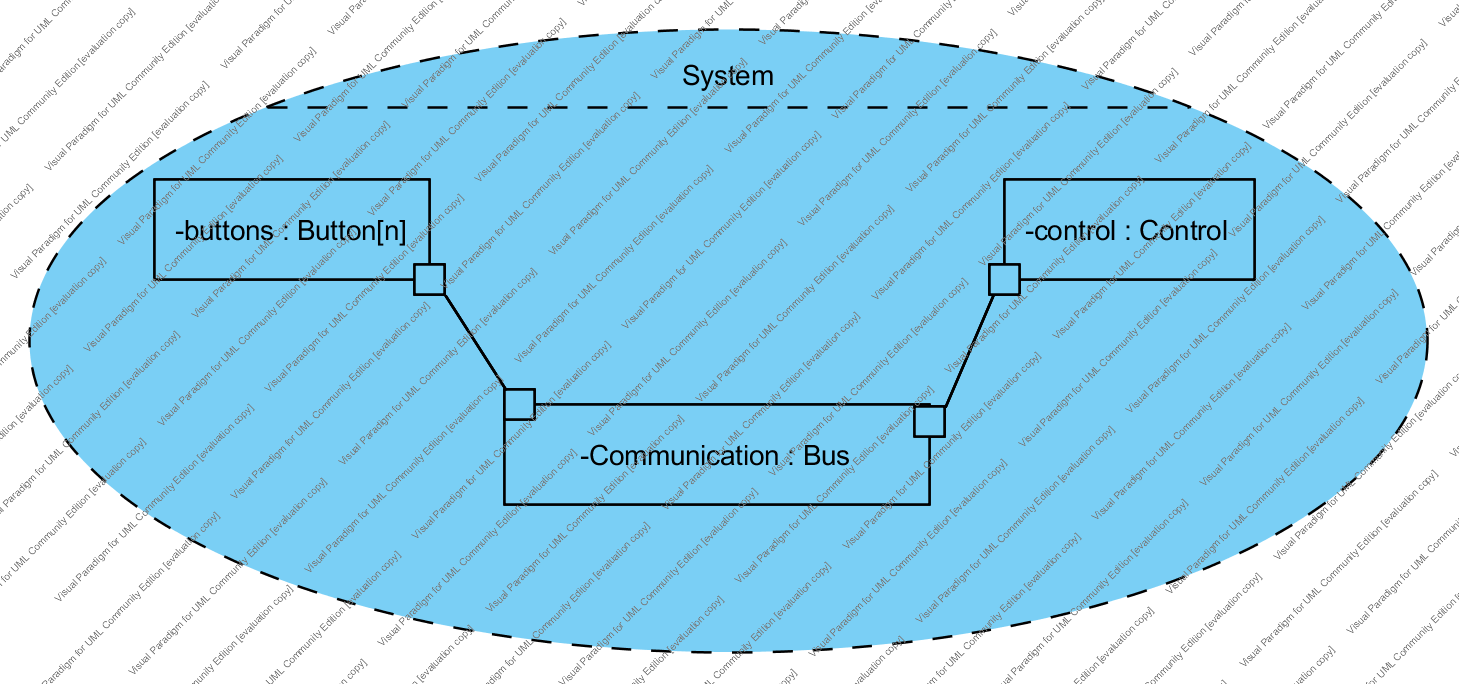
\includegraphics[width=\linewidth]{../comp1}
  \caption{Composite structure diagram, system from exercise 2}
  \label{fig:compex2}
\end{figure}

\begin{figure}[htbp]
  \centering
  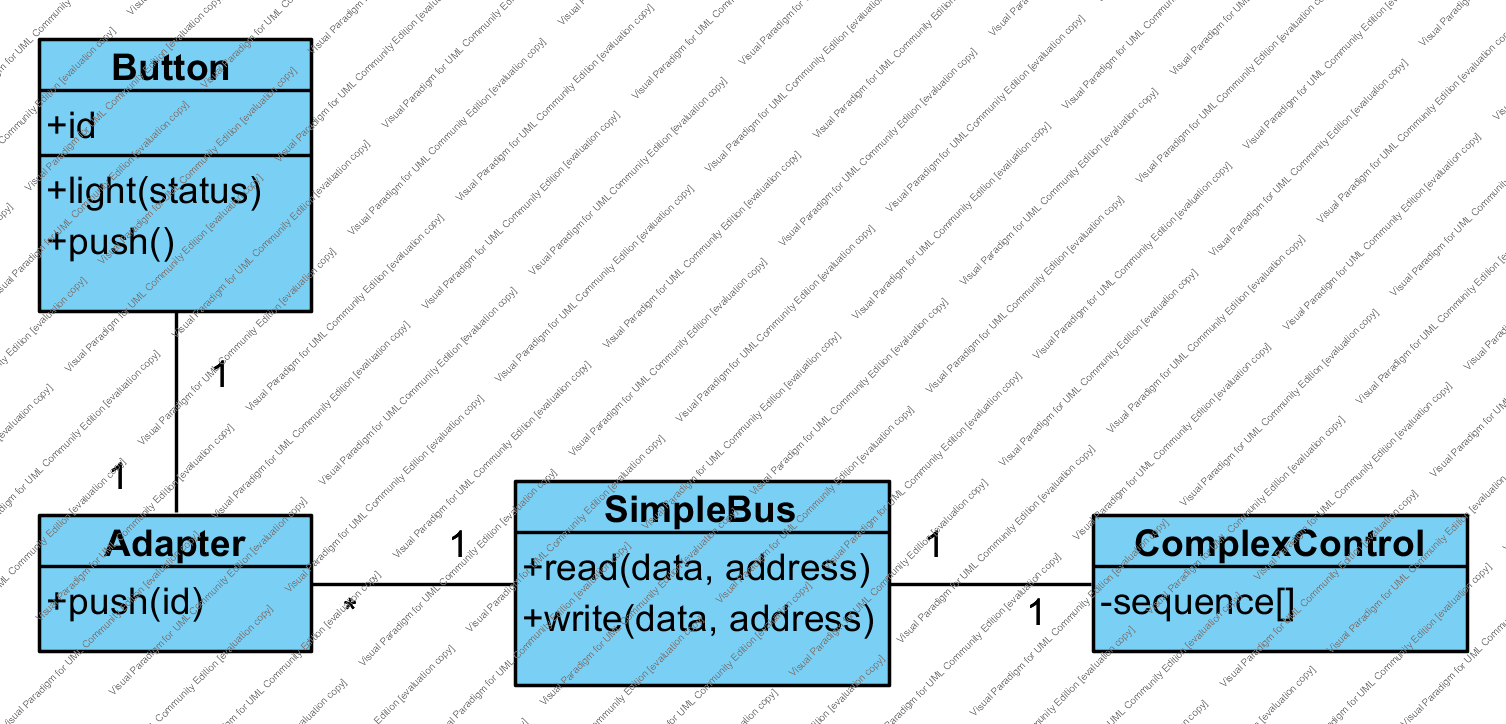
\includegraphics[width=0.8\linewidth]{../class3}
  \caption{Class diagram system from exercise 4}
  \label{fig:classex4}
\end{figure}
\begin{figure}[htbp]
  \centering
  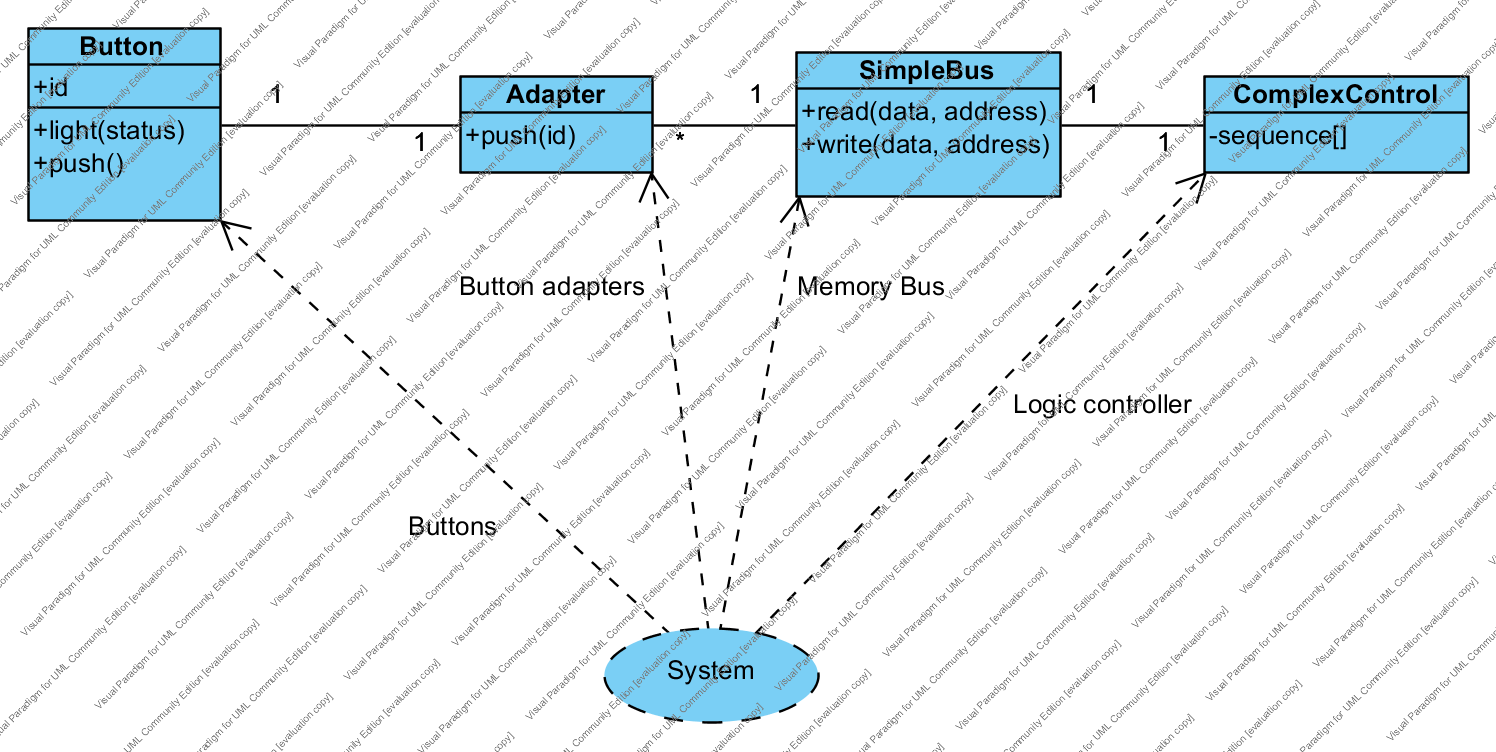
\includegraphics[width=\linewidth]{../class4}
  \caption{Collaboration use, system from exercise 4}
  \label{fig:collabex4}
\end{figure}

\begin{figure}[htbp]
  \centering
  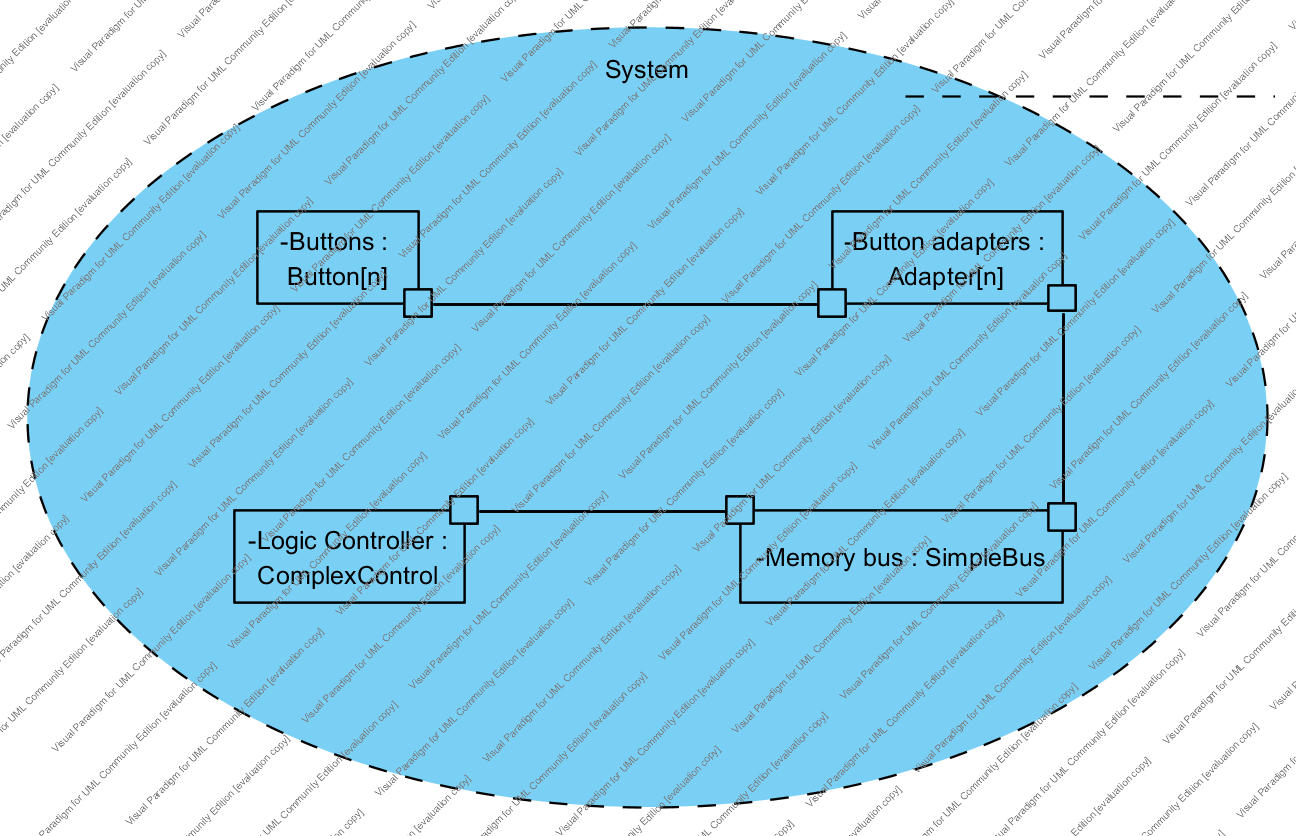
\includegraphics[width=\linewidth]{../comp2}
  \caption{Composite structure diagram, system from exercise 4}
  \label{fig:compex4}
\end{figure}
  

\section{State Machine Diagrams}
The state machine shown in figure \ref{fig:state} contains two concurrent states: One for the reset
state, and one for when the Memory Machine (the Controller) has received at
least one correct push, and is waiting for subsequent pushes. The initial state
takes the state machine to the reset state, without any function call/action
done. Since there is no defined end state, it has been omitted from the figure.
\begin{figure}[htbp]
  \centering
  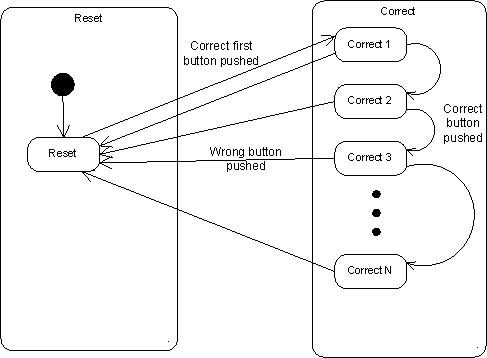
\includegraphics[width=\linewidth]{../state_hierarchical}
  \caption{State machine for the controller}
  \label{fig:state}
\end{figure}
  \end{document}
